\documentclass[runningheads]{llncs}

% =====================================================================
% COMPASS -- IJCKG 2026 submission
% IJCKG 2026 uses the Springer LNCS/LNAI format. The Research Track is the
% safer fit unless the authors can add documented evidence from target users.
% =====================================================================

\usepackage[T1]{fontenc}
\usepackage[utf8]{inputenc}

\usepackage{graphicx}
\usepackage{amsmath,amssymb}
\usepackage{booktabs}
\usepackage{enumitem}
\usepackage{placeins}
\usepackage[hidelinks]{hyperref}
\usepackage[strings]{underscore}

% ---- natbib-free compatibility shims ----
\providecommand{\citep}[1]{\cite{#1}}
\providecommand{\citet}[1]{\cite{#1}}

% Helper macro to input auto-generated LaTeX tables that contain underscores
\newcommand{\code}[1]{\texttt{\detokenize{#1}}}
\newcommand{\InputTableSanitized}[1]{%
  \begingroup\catcode`\_=12\relax\input{#1}\endgroup}

% Pretty mode / system names
\newcommand{\Compass}{\textsc{COMPASS}}
\newcommand{\BaseMode}{\textsc{Base}}
\newcommand{\MemMode}{\textsc{Mem}}
\newcommand{\MemSymMode}{\textsc{Mem+Sym}}
\newcommand{\RAGBase}{\textsc{RAG-Base}}
\newcommand{\SymOnly}{\textsc{Sym-Only}}
\newcommand{\RouterMode}{\textsc{Router}}
\newcommand{\RLMode}{\textsc{RL}}
\newcommand{\LongCtx}{\textsc{GPT-mini-Ret.}}
\newcommand{\LogicLM}{\textsc{Logic-LM-style}}
% Best configuration is COMPASS. The macro below keeps any legacy
% \AdaptiveRAG references compiling and rendering as COMPASS.
\newcommand{\AdaptiveRAG}{\textsc{COMPASS}}

\title{COMPASS: Reliable and Auditable Question Answering
for Digital Product Passports}
\titlerunning{COMPASS: Reliable and Auditable QA for Digital Product Passports}
% AUTHOR INPUT REQUIRED: add names, affiliations, email, and ORCIDs.
\author{}
\institute{}

\begin{document}
\maketitle

\begin{abstract}
Digital Product Passports (DPPs) expose product-level technical, compliance,
and sustainability information. Errors in this setting can affect audits,
purchasing decisions, and sustainability reports. A dependable
question-answering system should link each answer to evidence. It should also
withhold an answer when the required information is absent.

Retrieval-augmented and long-context large language models (LLMs) can answer
many factual questions from supplied text. Standard prompting alone, however,
does not ensure correct rule application, reuse of earlier session facts, or
consistent handling of missing evidence. We present \Compass, a DPP
question-answering architecture that either returns an answer or abstains. It
combines document retrieval, session-scoped text memory, and targeted rules
over structured product facts. The rules operate on a DPP ontology informed by
CIRPASS-2 requirements. Each released study retains the answer path and the
evidence fields saved by its runner. The current endpoint has no shared online
confidence threshold, so we analyze selective decisions only after inference.

We evaluate \Compass\ on a verified subset of a template-generated DPP-like
benchmark with 6,270 questions. A second controlled benchmark contains 3,000
questions that combine document, memory, and structured evidence. A separate study
supplies the relevant Open Food Facts row for each of 4,021 queries. On the
verified benchmark, \Compass\ reaches 0.9998 accuracy, compared with 0.9702 for
the strongest external baseline. This is a full-system comparison:
6,266 outputs use deterministic document or symbolic graph paths, while four
use the LLM fallback. The complete system also answers every compositional
question correctly. In the Open Food Facts study, later text-based rescoring
identifies explicit missing-evidence responses that the original JSON
abstention flag misses.

All three prompting baselines score below \Compass\ on both controlled
benchmarks. These results are limited to the released tasks and do not
establish performance on unrestricted natural queries or in production. We
release the ontology, rules, benchmark generators, evaluation code, and
per-item outputs for the two frozen benchmarks.
\end{abstract}

\keywords{Digital Product Passports \and question answering \and retrieval
\and symbolic reasoning \and abstention}

\section{Introduction}
Digital Product Passports (DPPs) make product information available across a
product's life cycle \cite{eu2024espr}. A passport may contain a
technical specification, a material record, an environmental value, or
evidence related to a standard. People use these records for audits,
procurement, repair, and sustainability reporting. In such settings, a fluent
answer is not enough. The reader must be able to inspect its evidence. When
the record does not support an answer, the system should say so.

Three problems make this task harder than ordinary document search. First,
evidence may be split across files and earlier messages in the same session.
Second, some questions ask for a consequence of several facts. The answer must
then be derived by a rule rather than copied from a passage. Third, product
records are incomplete. Missing or conflicting evidence should lead to an
abstention, not a plausible guess.

Long-context prompting and retrieval-augmented generation (RAG) address part
of this problem. RAG selects passages and gives them to a large language model
(LLM) before it answers. A long prompt can instead hold more of the record at
once. Neither method guarantees that the model will use the right passage.
Evidence in the middle of a long prompt is often neglected
\cite{liu2024lostinthemiddle}. A natural-language explanation can also differ
from the process that produced the answer
\cite{turpin2023unfaithfulcot}. Retrieval alone does
not evaluate a compliance rule or decide how missing evidence should be
handled.

\Compass\ combines three limited and complementary sources. Document retrieval
finds relevant passages. Session memory retrieves text saved earlier in the
same interaction. A symbolic layer looks up graph facts and applies a small
set of targeted rules. The graph is not a replacement for the documents.
Runtime responses expose path and evidence fields when available; the frozen
studies retain different subsets of those fields. We study answer coverage,
error, and calibration only where a score was saved
\cite{kamath2020selectiveqa,guo2017calibration,traub2024aurc}.

We developed \Compass\ within CE-RISE, an EU Horizon Europe project on
circular-resource information systems. The released evaluation material uses
curated DPP-like seed records for batteries, printing hardware, and heating
systems. The workbench has been shown to consortium practitioners outside the
development team. Those sessions were not logged in enough detail to support
a user study.

\noindent Our contributions are:
\begin{itemize}[leftmargin=1.2em,itemsep=2pt,topsep=2pt]
  \item We present an answer-or-abstain interface for DPP question answering.
  It combines document retrieval, same-session memory, graph lookup, and
  targeted derivation while exposing path and available evidence fields.
  \item We give a reliability evaluation that separates correctness,
  risk under abstention, confidence calibration, and symbolic-path use. It
  includes paired comparisons on identical questions
  \cite{wilson1927probable,mcnemar1947note}.
  \item We release two frozen, template-generated benchmarks and their
  item-level predictions: 6,270 verified DPP-like questions and 3,000
  controlled composition questions. We also report a field-aware abstention
  study with 4,021 Open Food Facts queries.
\end{itemize}

\section{Related work}

\paragraph{Retrieval and long context.}
RAG conditions a generated answer on retrieved passages
\cite{lewis2020rag}. It improves access to source text, but does not make the
source complete or the answer logically valid. Longer contexts remain
sensitive to where evidence appears \cite{liu2024lostinthemiddle}. \Compass\
keeps retrieval for document questions. A separate symbolic path handles
graph lookup and the limited facts derived from the structured record.

\paragraph{External memory.}
Prior work retrieves information outside model parameters or carries state
across text segments \cite{khandelwal2020knnlm,bulatov2022rmt}. Our memory has
a smaller role. It stores timestamped text within one session. It is not a
verified product database. Durable use would require product isolation,
source validation, and a correction history.

\paragraph{Ontologies and rules.}
An ontology names the entities and relations in a domain. The Web Ontology
Language (OWL) also supports rule-based inference over those relations.
Restricted OWL profiles make this inference practical
\cite{motik2009owl2profiles}. Neurosymbolic systems pair learned models with
explicit rules or solvers. LINC and Logic-LM, for example, couple an LLM to
symbolic inference \cite{olausson2023linc,pan2023logiclm}. Our comparison systems reproduce
their prompting style, not their complete published solvers. \Compass\ uses a
narrower symbolic layer. It looks up or derives selected DPP facts and leaves
ordinary document questions to retrieval.

\paragraph{Abstention and confidence.}
Selective prediction studies when a model should answer and when it should
abstain \cite{kamath2020selectiveqa}. A
risk--coverage curve shows the price of answering more questions, while AURC
summarizes that curve \cite{traub2024aurc}. Calibration asks a different
question: whether a score such as 0.8 corresponds to about 80\% correctness
\cite{guo2017calibration}. \Compass\ records a heuristic
score. We test its ranking and calibration separately. We do not treat it as
a probability merely because it lies between zero and one.

\section{Problem formulation and metrics}
For $N$ evaluated questions, let $x_i$ be question $i$ and $E_i$ its available
document, memory, and structured evidence. The answer component is
$y_i=f(x_i,E_i)$. It may be $\bot$, meaning that it is withheld. Trace fields
differ by path and release. When a study retains a score $c_i\in[0,1]$, we
treat it as a heuristic rather than an assumed probability. Applying an
offline threshold $\tau$ yields

\[
\widetilde y_{\tau}(x_i)=
\begin{cases}
  y_i, & y_i\neq\bot\ \text{and}\ c_i\geq\tau,\\
  \bot, & y_i=\bot\ \text{or}\ c_i<\tau.
\end{cases}
\tag{1}
\]

Here, raising $\tau$ withholds more low-scoring answers. We vary it only after
inference. The endpoint does not use a fitted calibrator or one shared
production threshold.

Let $z_i=1$ when the scorer marks the whole output correct, and $z_i=0$
otherwise. In an answerability test, a required abstention can therefore have
$z_i=1$. Let $A_{\tau}=\{i:y_i\neq\bot,\ c_i\geq\tau\}$ be the answered set.
Then

\[
\operatorname{Coverage}(\tau)=\frac{|A_{\tau}|}{N},
\qquad
\operatorname{Risk}(\tau)=
\frac{\sum_{i\in A_{\tau}}(1-z_i)}{|A_{\tau}|}.
\tag{2}
\]

Coverage is the fraction answered. Risk is the error rate among those answers.
Thus, coverage 0.80 and risk 0.05 mean that 80 of 100 questions are answered
and four of those answers are wrong. Risk requires a nonempty $A_{\tau}$.

A risk--coverage curve plots these two quantities as $\tau$ changes. Its area
is

\[
\operatorname{AURC}=\int_{0}^{1}\operatorname{Risk}(u)\,du,
\tag{3}
\]

where $u$ denotes coverage. We use trapezoids at the unique stored scores. For
the zero-coverage boundary, the calculation carries back the risk at the first
attainable threshold; that boundary is a numerical convention, not an observed
operating point. A lower AURC means that errors tend to receive lower scores
and are removed earlier. It does not establish calibration
\cite{kamath2020selectiveqa,traub2024aurc}.

Some benchmarks label each question as answerable or unanswerable.
\emph{Decision accuracy} credits a correct answer to an answerable question or
a correct abstention otherwise. \emph{Answer accuracy} is the fraction correct
among answered questions. Abstention precision is the fraction of abstentions that were
required. Abstention recall is the fraction of required abstentions made.
Together, they expose a system that gains accuracy merely by refusing most
questions.

Expected calibration error (ECE) tests whether scores match observed
correctness. Divide the outputs into $B$ score bins $I_b$. Let
$\operatorname{acc}(I_b)$ and $\operatorname{conf}(I_b)$ be the mean
correctness and score in bin $b$. We use

\[
\begin{aligned}
\operatorname{ECE}&=\sum_{b=1}^{B}\frac{|I_b|}{N}
 \left|\operatorname{acc}(I_b)-\operatorname{conf}(I_b)\right|,\\
\operatorname{Brier}&=\frac{1}{N}\sum_{i=1}^{N}(c_i-z_i)^2.
\end{aligned}
\tag{4}
\]

If outputs near 0.8 confidence are correct only half the time, the score is
overconfident in that bin. ECE depends on how bins are formed, so we report
equal-count and fixed-width variants where available. Brier is the mean
squared distance between score and correctness. Lower values are better
\cite{guo2017calibration}.

Wilson 95\% intervals summarize uncertainty around observed accuracy and
remain well behaved near zero or one \cite{wilson1927probable}. McNemar's
exact test compares two systems on the same questions by counting rows won
only by each system \cite{mcnemar1947note}. Repeated templates limit how far
either result can be generalized. Symbolic-path coverage is the
fraction of rows marked as using a symbolic step. Symbolic-path accuracy is
accuracy within that subset. Because the mark omits the exact rule and its
premises, it is not individual-rule precision.

\section{The COMPASS architecture}

\subsection{Design principles and inference path}
Figure~\ref{fig:architecture} separates evidence acquisition from answer
construction. Retrieval, same-session memory, and the symbolic graph provide
candidate evidence. The verified path returns a document field, a looked-up
graph fact, or a derived fact when available. It uses the LLM otherwise. The
composition path asks the LLM to combine evidence; deterministic checks may
supplement or replace its draft. The LLM is prompted to cite its context, but
this cannot ensure that it ignores prior knowledge.

The frozen artifacts retain different trace fields. Verified rows keep a path
label and either document identifiers or graph evidence, plus a stored score.
Composition rows keep LLM path and model metadata, but no common confidence
field and often no selected evidence identifiers. Figure~\ref{fig:architecture}
therefore shows available release fields rather than a complete audit log.

\begin{figure}[h]
\centering
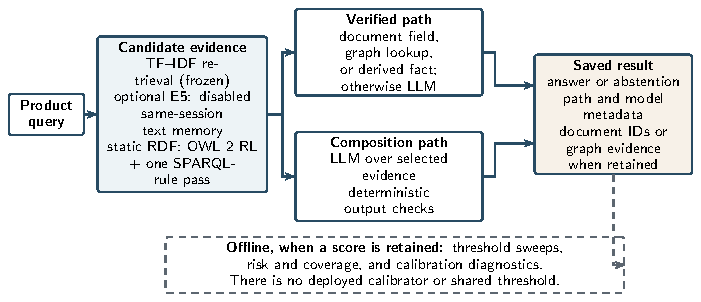
\includegraphics[width=0.88\linewidth]{figures/compass_architecture.pdf}
\caption{The two frozen evaluation paths and available trace fields. Evidence
and confidence fields vary by release. Dashed analysis occurs after inference
and only where a score is retained.}
\label{fig:architecture}
\end{figure}

\subsection{Evidence acquisition: document retrieval and session memory}
The retriever always computes a TF--IDF score. The runtime can optionally add
an E5 meaning-based score \cite{wang2022e5}. For query $x$ and candidate
passage $d_j$, the optional hybrid score is

\[
s(x,d_j)=\tfrac{1}{2}\operatorname{zscore}\!\left(s_{\mathrm{TFIDF}}(x,d_j)\right)
 +\tfrac{1}{2}\operatorname{zscore}\!\left(s_{\mathrm{E5}}(x,d_j)\right),
\quad
\operatorname{zscore}(s_j)=\frac{s_j-\bar{s}}{\sigma_s}.
\tag{5}
\]

TF--IDF measures word overlap while giving more weight to words that are
uncommon in the corpus. E5 represents the query and passage as vectors, so it
can match similar meanings expressed with different words. Their raw score
ranges differ. The mean $\bar{s}$ and standard deviation $\sigma_s$ are taken
over the indexed passages for the query; zero variance uses a divisor of one.
This standardization prevents one scale from dominating. Both frozen
benchmark runners explicitly disabled E5 and ranked passages by TF--IDF alone.
The reported results therefore do not measure the optional hybrid blend.
Neither frozen runner reranks the retrieved passages.

Session memory stores timestamped text and retrieves it within the same
session. It uses cosine similarity, which measures closeness between embedding
vectors. The answerer is prompted to cite passage identifiers. If an LLM
answer lacks a bracketed citation, the wrapper appends the first identifier.
This enforces format, not support for each claim. The runtime can return
identifiers, scores, snippets, and the answer path, but it does not keep an
immutable copy of the full prompt.

The current memory can mix entries from different products in one session. It
does not verify the source of an entry or preserve an append-only correction
history. A production deployment needs all three controls.

\subsection{Targeted symbolic reasoning over a DPP ontology}
Some questions require a derived answer. A product may require a standard
because it contains a certain component. The symbolic layer handles this
limited class of questions.

\emph{Fact graph.} The service loads structured facts from released RDF
files. It does not extract them from session memory at query time. Each fact
is a Resource Description Framework (RDF) triple. A triple has a subject, a
predicate, and an object. For example, $(P,\texttt{hasComponent},C)$ states
that product $P$ contains component $C$.

\emph{Ontology.} The core vocabulary covers products, components, materials,
process steps, and standards. Domain files provide battery, printing,
heating, and textile terms. The vocabulary is informed by the
CIRPASS-2 requirements specification \cite{cirpass2}. Its mapping links are
descriptive. They do not assert logical equivalence.

\emph{Rules.} The implementation uses a finite set of domain-specific SPARQL
\texttt{CONSTRUCT} rules. SPARQL is a query language for RDF data. One battery
rule is:
\[
\begin{aligned}
\texttt{hasComponent}(p,c) \wedge
\texttt{rdf:type}(c,\texttt{Battery})\\
{}\Rightarrow
\texttt{requiresCompliance}(p,\texttt{BatterySafetyStandard}).
\end{aligned}
\tag{6}
\]
Here, $p$ stands for a product and $c$ for one of its components. The first
statement says that $p$ contains $c$. The RDF type statement says that $c$ is
a battery. The symbol $\wedge$ means that both statements must hold. The arrow
then adds the conclusion on the right: the product requires the named battery
safety standard. This is one derived graph fact. It is not, by itself, a legal
finding or a complete proof of compliance.

At startup, the service expands the static graph under OWL~2~RL, a restricted
OWL profile designed for efficient rule-based inference
\cite{motik2009owl2profiles}. It then applies the SPARQL rule list once. It
does not repeat the rules until no new facts appear.

\emph{Missing facts.} OWL uses an open-world assumption. An absent triple is
therefore unknown rather than false. Some released rules use
\texttt{FILTER NOT EXISTS}. This is a local check for a required process step
that is not recorded in the loaded graph. The reasoner does not provide
general checks for missing fields, stale reports, or date windows.

\emph{Recorded evidence.} Rule-derived responses record standards or process
steps when present. Symbolic responses also record that the symbolic path was
used. They do not retain every matched premise or the exact SPARQL rule
identifier. The record supports inspection, but not reconstruction of the full
proof. Historical symbolic-path coverage and accuracy appear in
Section~\ref{sec:historical}.

\subsection{Confidence, calibration, and operating modes}
The runtime attaches a hand-designed confidence score to each answer. A memory
path uses its top similarity score, clipped to $[0,1]$. A retrieval path maps
its top search score to the $0$--$1$ range with an S-shaped function. A
symbolic path uses an explicit verdict score when one is available. Otherwise,
it uses 0.5. When several paths contribute, the implementation keeps the
largest score. It does not use snippet agreement or token-generation
probabilities.

On every pooled row, \texttt{confidence\_cal} equals the raw score. No fitted
calibration map is recoverable. We therefore evaluate the stored scores as
they are. After the answers are produced, we vary the threshold $\tau$ and
plot risk against coverage. The online endpoint has no calibration model or
shared threshold. The Open Food Facts study also uses the model's reported
confidence without fitting a later calibration model.

The pooled study also reports configurations that isolate parts of the system.
\RAGBase\ uses retrieval only. \MemMode\ uses memory only. \SymOnly\ uses the
symbolic graph path. \MemSymMode\ combines memory and that path. \RouterMode\
uses the learned router. The experimental \RLMode\ uses reinforcement
learning (RL). The verified release records the project system as
\texttt{ADAPTIVERAG}. The composition study
records its full evidence-combining mode as \texttt{AUTO\_COMPOSE}. Both modes
appear as \Compass\ in the paper, while the release keeps their internal
names.

\section{Experimental setting}
\subsection{Studies and data}
The main DPP study uses 6,270 items from a frozen, template-generated DPP-like
benchmark. It contains 2,649 logic questions, 871 open-extraction questions,
and 2,750 recall questions. The generator uses the released ontology and
curated seed records for batteries, printing hardware, and heating systems.
This is not a natural-query or regulatory DPP corpus. Fixed filters remove
malformed labels, ambiguous or unsupported reference answers, and conflicting
graph relations. The filters do not inspect system predictions.

The second study is a controlled, generated benchmark with 3,000 questions.
Its six subtypes require document evidence, session memory, structured facts,
or combinations of these sources. The third study uses 4,021 Open Food Facts
queries \cite{openfoodfacts}. It covers nutrition, product attributes, missing
fields, sustainability, and fairness. The answerer receives the relevant
product row or aggregate missingness row. Its prompt also names the fields
needed by the query.

We also report an archived, template-generated DPP-like run with 3,429
questions. It predates the frozen release. Of these, 295 are logic questions,
2,297 are open questions, and 837 are recall questions. We use this run only
for internal component comparisons, symbolic-path coverage, and selective
analysis. We could not rerun it because 2,084 rows lack recoverable reference
labels.

The verified release uses deterministic scoring for each question type. A
logic answer must agree with the expected yes/no label. For open and recall
questions, the scorer normalizes the text and checks for the expected answer.
The composition study requires at least one accepted value from
every expected source group. Open Food Facts uses missing-field labels and
normalized text matching. Numeric answers allow the larger of 0.01 or 0.5\%
error. Percentages allow 0.25 percentage points. No study uses an LLM judge.

Both frozen benchmarks repeat question forms and source entities. After
replacing product identifiers and numbers, the verified set has 289 distinct
question forms and the composition set has 497. Wilson intervals and row-level
McNemar tests therefore describe the observed benchmark items. They do not
justify claims about a wider population of independent, naturally occurring
queries.

Both frozen DPP benchmarks contain supported, answerable items. They do not
test native abstention decisions. Abstention evidence comes from the offline
archived analysis and the separately rescored Open Food Facts study.

\subsection{Baselines}
The pooled suite uses \RAGBase\ and the internal component comparisons. The
frozen studies add three GPT-4o-mini baselines. \LongCtx\ denotes GPT-4o-mini
with retrieved context. It receives
up to 12,000 selected characters \cite{liu2024lostinthemiddle}. A
Logic-LM-style prompt asks for classification and reasoning
\cite{pan2023logiclm}. A LINC-style prompt supplies a premise, goal, and
reasoning instruction \cite{olausson2023linc}. The last two are approximations.
They do not run the full published solver systems.

The three external baselines and all model calls in the composition study
resolve to \texttt{gpt-4o-mini-2024-07-18}. The systems use the same questions
and scoring rules within each study. The release includes prompts, decoding
settings, evidence budgets, predictions, and known departures from the
published baseline procedures. The older Open Food Facts run retains only the
\texttt{gpt-4o-mini} alias. Its dated model version was not saved.

The composition harness supplies the benchmark's declared evidence sections.
External baseline configurations mark this as oracle context
and use gold source groups to select document, memory, and structured values.
The comparison therefore tests composition given relevant evidence. It does
not test end-to-end retrieval or source routing.

\section{Results}
\label{sec:results}
\subsection{Frozen verified release}
\label{sec:verified}
The frozen release contains 2,649 logic questions among 6,270 questions in
total. \Compass\ answers 6,269 questions correctly. Its accuracy is 0.9998, with a
Wilson 95\% interval of [0.9991, 1.0000]. \LogicLM\ scores 0.9702,
\LongCtx\ 0.9662, and the LINC-style baseline 0.9512
(Table~\ref{tab:verified}). The result is also stable across the three source
domains: 1,268 of 1,269 battery items and every printing-hardware and
heating-system item are correct.

The item-level paired tests use the same 6,270 rows for every system. The
numbers of \Compass-only/baseline-only wins are 212/1 against \LongCtx, 306/1
against LINC-style, and 187/1 against \LogicLM. Every exact McNemar test has
$p<10^{-10}$. These results show near-perfect item accuracy on this controlled
subset. They do not show that DPP question answering is solved.

This is a system-level comparison. The saved \Compass\ paths mark 5,265
outputs as symbolic, 1,001 as direct field extraction, and four as LLM
fallbacks. Within the symbolic group, trace labels mark 2,649 class-membership
lookups, 2,594 knowledge-base recalls, 14 component lookups, and eight rows
carrying both compliance and required-step labels. These are path labels, not
retained proofs of individual custom-rule executions. The comparison therefore
evaluates complete systems, not two prompts with equal model use.

Every verified \Compass\ row stores confidence 0.5. This release cannot support
a risk ranking or calibration analysis. The composition package has no common
confidence field. Selective-risk and calibration evidence is therefore limited
to the archived pooled run and Open Food Facts study below.

The only \Compass\ error is a generated open-extraction item. Its question
combines the labels ``Natural convection'' and ``Enclosure.'' The system
returns ``Natural convection,'' while the reference expects the enclosure
rating ``IP20.'' The case exposes a remaining boundary problem between nearby
template fields rather than a missing document.

\begin{table}[h]
\centering
\caption{Item accuracy on the verified release ($n{=}6270$). All systems use
the same questions and scoring rules. The last column gives
\Compass-only/baseline-only wins. All item-level exact McNemar tests have
$p<10^{-10}$.}
\label{tab:verified}
\footnotesize
\setlength{\tabcolsep}{4pt}
\renewcommand{\arraystretch}{1.0}
\begin{tabular}{lcccccc}
\toprule
Method & Acc. & 95\% CI & Logic & Open & Recall & McNemar \\
\midrule
\Compass & \textbf{0.9998} & [0.9991, 1.0000] & 1.0000 & 0.9989 & 1.0000 & --- \\
\LogicLM & 0.9702 & [0.9657, 0.9741] & 0.9370 & 0.9782 & 0.9996 & 187 / 1 \\
\LongCtx & 0.9662 & [0.9614, 0.9704] & 0.9332 & 0.9633 & 0.9989 & 212 / 1 \\
LINC-style & 0.9512 & [0.9456, 0.9563] & 0.9566 & 0.9208 & 0.9556 & 306 / 1 \\
\bottomrule
\end{tabular}
\end{table}

\subsection{Controlled compositional benchmark}
\label{sec:composition}
The release names the full \Compass\ configuration \texttt{AUTO\_COMPOSE}.
It answers all 3,000 benchmark questions correctly. \LongCtx\ answers 2,878
(0.9593). \LogicLM\ answers 2,822 (0.9407), and LINC-style answers 2,672
(0.8907).

\texttt{AUTO\_COMPOSE} attempted an LLM call on every row. Deterministic output
checks then changed or supplemented 198 answers. In 20 final traces, the LLM
answer was discarded. The 1.0000 score belongs to this full system, not to
the LLM alone.

The largest gap occurs on the 225 questions that require memory, document,
and symbolic evidence. Accuracies on this subtype are 1.000 for \Compass,
0.707 for \LongCtx, 0.631 for \LogicLM, and 0.524 for LINC-style. The
document--memory subtype also separates the systems. By contrast, all
baselines are near perfect on several memory--symbolic subtypes. Every
item-level paired test against \Compass\ has $p<10^{-36}$.

This generated benchmark measures composition from supplied evidence. It does
not test retrieval or naturally occurring queries.

\begin{table}[h]
\centering
\caption{Accuracy on the 3,000-question compositional benchmark. The largest
gap occurs when a question needs document, memory, and structured evidence.}
\label{tab:arch}
\footnotesize
\setlength{\tabcolsep}{3pt}
\renewcommand{\arraystretch}{1.0}
\begin{tabular}{lcccc}
\toprule
Subtype & \Compass & \shortstack{GPT-4o-mini\\retrieved} &
\shortstack{LINC-\\style} & \shortstack{Logic-LM-\\style} \\
\midrule
Overall (3000) & \textbf{1.000} & 0.959 & 0.891 & 0.941 \\
\midrule
Atomic verified (1500) & 1.000 & 0.984 & 0.913 & 0.973 \\
Document + memory (225) & 1.000 & 0.867 & 0.702 & 0.760 \\
Doc. + memory + structured (225) & 1.000 & 0.707 & 0.524 & 0.631 \\
Memory + struct.: compliance (375) & 1.000 & 1.000 & 0.968 & 1.000 \\
Memory + struct.: component (375) & 1.000 & 0.995 & 0.971 & 1.000 \\
Memory + struct.: process (300) & 1.000 & 1.000 & 1.000 & 1.000 \\
\bottomrule
\end{tabular}
\end{table}

\subsection{Field-aware abstention on Open Food Facts}
\label{sec:off}
We evaluate a GPT-4o-mini answerer given row context from Open Food Facts. The
data uses a different schema. The answerer receives the relevant product row
or aggregate missingness row. Its prompt also names the fields required by the
query. This is a field-aware row-context test. It does not evaluate
retrieval over the raw data dump or transfer of the symbolic reasoner. A direct
lookup is labeled unanswerable when its required field is absent. A missingness
question asks whether a field is present, so it remains answerable.

On 4,021 queries, decision accuracy is 0.972. Answer accuracy is 0.963 at
0.730 coverage (Table~\ref{tab:off}). Fixed-width-bin ECE is 0.021. These
figures use a text-based rule applied after generation during rescoring. It
treats answers such as ``Missing'' or ``Insufficient context'' as abstentions,
even when the model's JSON flag says otherwise. Missingness questions are
exempt because ``missing'' is a valid factual answer. The raw flag marks 385
abstentions. Its recall against the unanswerable labels is 0.353. The
text-based rule reclassifies 702 more outputs, producing 1,087 abstentions. Of
these, 1,085 match the unanswerable labels. Effective abstention precision is
0.998 and recall is 1.000.
Sustainability is the weakest category. Its answer accuracy is 0.787 at 0.380
coverage. The fairness subset has only 19 questions. It is too small to
support a separate claim.

\begin{table}[t]
\centering
\caption{Results on Open Food Facts ($n{=}4021$) after text-based abstention
rescoring. Decision accuracy credits a correct answer or abstention.
Answer accuracy covers answered queries only. ECE uses ten fixed-width bins
and post-rescoring decision correctness.}
\label{tab:off}
\footnotesize
\setlength{\tabcolsep}{4pt}
\renewcommand{\arraystretch}{1.0}
\begin{tabular}{lccccc}
\toprule
Query type & $n$ & Dec.\ acc. & Ans.\ acc. & Coverage & ECE \\
\midrule
All & 4021 & 0.972 & 0.963 & 0.730 & 0.021 \\
\midrule
nutrition & 1450 & 1.000 & 1.000 & 0.696 & 0.004 \\
attribute & 1146 & 0.998 & 1.000 & 0.998 & 0.002 \\
missingness & 367 & 0.929 & 0.929 & 1.000 & 0.071 \\
sustainability & 1039 & 0.919 & 0.787 & 0.380 & 0.060 \\
fairness & 19 & 1.000 & 1.000 & 1.000 & 0.000 \\
\bottomrule
\end{tabular}
\end{table}

\FloatBarrier
\subsection{Historical component comparison}
\label{sec:historical}
Table~\ref{tab:summary} summarizes an archived run on 3,429 questions. It is
not part of the frozen external-baseline comparison. Saved outputs contain an
answer for every row. \Compass\ records 0.9749 accuracy and AURC 0.0115.
\RAGBase\ records 0.8973 accuracy and AURC 0.1027. \Compass\ alone is correct
on 266 paired rows. \RAGBase\ alone is correct on none ($p<10^{-6}$).
\Compass\ receives retrieved evidence plus memory and symbolic pathways. The
comparison therefore does not isolate a single causal mechanism.

\begin{table}[h]
\centering
\caption{Archived component and query-type results ($n{=}3429$). AURC uses
every unique score. Dashes mark modes omitted from that calculation.}
\label{tab:summary}
\footnotesize
\setlength{\tabcolsep}{2.6pt}
\renewcommand{\arraystretch}{1.0}
\begin{tabular}{lcccccc}
\toprule
Method & Acc. & 95\% CI & AURC & Logic & Open & Recall \\
\midrule
\Compass & 0.9749 & [0.9691, 0.9796] & 0.0115 & 0.7085 & 1.0000 & 1.0000 \\
\RAGBase & 0.8973 & [0.8867, 0.9071] & 0.1027 & 0.0102 & 1.0000 & 0.9283 \\
\RLMode & 0.8965 & [0.8858, 0.9062] & 0.4220 & 0.0034 & 1.0000 & 0.9271 \\
\MemSymMode & 0.5777 & [0.5611, 0.5942] & 0.1377 & 0.7085 & 0.5320 & 0.6571 \\
\MemMode & 0.5001 & [0.4834, 0.5169] & -- & 0.0136 & 0.5320 & 0.5842 \\
\SymOnly & 0.0965 & [0.0871, 0.1069] & 0.4158 & 0.9051 & 0.0000 & 0.0765 \\
\RouterMode & 0.0869 & [0.0779, 0.0968] & 0.4269 & 0.7932 & 0.0000 & 0.0765 \\
\BaseMode & 0.0169 & [0.0131, 0.0218] & -- & 0.1966 & 0.0000 & 0.0000 \\
\bottomrule
\end{tabular}
\end{table}

At full coverage, observed risk is 0.0251 for \Compass\ and 0.1027 for
\RAGBase. Thresholding \Compass's confidence produces lower-coverage points,
including points with no observed error. The archived \RAGBase\ confidence is
constant. It therefore yields only one attainable point, at full coverage.
Figure~\ref{fig:riskcov} does not establish dominance across a shared range of
thresholds.

Open and recall questions are saturated in this run. They offer little
separation between architectures. On logic questions, \Compass\ scores 0.7085
and \RAGBase\ 0.0102. \SymOnly\ scores 0.9051 on logic, but only 0.0965
overall. The archived table marks 273 \Compass\ rows (7.96\%) as symbolic-path
cases. All 273 associated final answers are labeled correct. Symbolic-path
accuracy is therefore 1.000, with an item-level Wilson 95\% interval of [0.986,
1.000]. The retained table does not identify exact rule executions or their
premises. This interval describes final-answer accuracy among symbolically
marked rows. It does not estimate the precision of individual SPARQL rules.

\begin{figure}[h]
\centering
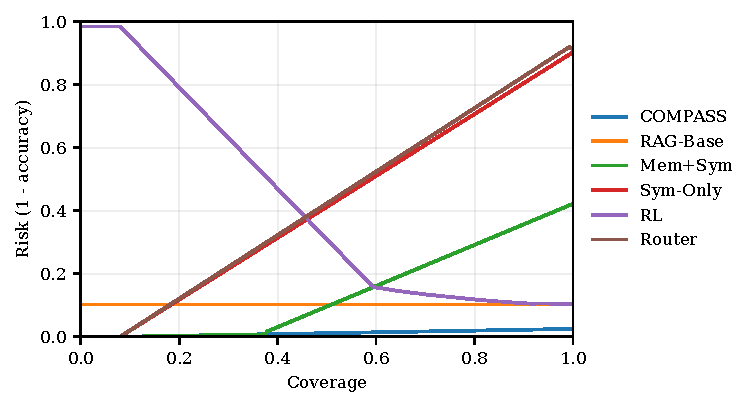
\includegraphics[width=0.58\linewidth]{artifacts/risk_coverage.pdf}
\caption{Risk--coverage curves from the archived pooled run. \RAGBase\ has
one tied confidence value, so only its full-coverage endpoint is attainable.
The line from zero coverage is drawn only to calculate AURC.}
\label{fig:riskcov}
\end{figure}

\section{Discussion and limitations}
\label{sec:disc}
\paragraph{Interpretation.}
The two frozen studies provide the strongest evidence. In the verified study,
most \Compass\ outputs follow deterministic document or graph paths. In the
composition study, the largest gap appears when supplied evidence spans
documents, memory, and structured facts. The archived run is secondary because
2,084 reference labels cannot be recovered. Its 273 symbolic-path cases are
all correct, but they do not isolate individual rule effects.

\paragraph{Calibration.}
High accuracy does not imply reliable probabilities. The archived field named
\texttt{confidence\_cal} is identical to the raw score and should not be read as
a calibrated probability. Equal-count bins contain
similar numbers of predictions. Fixed-width bins divide the confidence range
into equal intervals. With equal-count bins, ECE is 0.5247 for \Compass\ on the
archived run. A row bootstrap, which resamples saved rows with replacement,
gives a 95\% interval of [0.5181, 0.5311]. Its Brier score is 0.3165.
\RAGBase\ has ECE 0.4873, interval [0.4771, 0.4967], and is also poorly
calibrated. Open Food Facts has equal-count ECE 0.0328, interval [0.0276,
0.0377], Brier 0.0287, and fixed-width ECE 0.021. Because templates repeat,
the intervals describe saved rows rather than a population of natural
queries. The tasks also differ, so calibration does not necessarily transfer.

\paragraph{Filtering and validator checks.}
\label{sec:filtering}
The verified filter removes 645 of 6,915 rows. It checks source support,
ambiguity, and whether each reference answer is a single value. It does not
read system predictions. A retained audit scores the same saved outputs before
and after filtering. Accuracy changes from 0.9721 to 0.9998 for \Compass,
0.9424 to 0.9657 for \LongCtx, 0.9202 to
0.9488 for LINC-style, and 0.9503 to 0.9699 for \LogicLM. The baseline scores
in Table~\ref{tab:verified} come from the later frozen rerun and are slightly
different. Filtering improves every system in the same-output audit. The gain
from filtering is not unique to \Compass. Not every source file for this diagnostic is in the
frozen package, so the summary cannot be fully recomputed from that package.

The current deterministic scorer reproduces the archived decisions for a
sample of 100 errors drawn roughly equally from the three external baselines.
Manual review nevertheless identifies 12 likely false negatives. In these
cases, the exact-span rule rejects an answer that omits an expected qualifier. This small audit
does not establish the scorer's overall error rate. Static code
inspection finds no imports between the question generator and runtime rule
modules. They share the released ontology and seed data by design.

\paragraph{In-use evidence.}
The CE-RISE workbench has been demonstrated to consortium practitioners
outside the development team. It shows retrieved passages, session memory,
derived triples, raw confidence, and the selected answer path. We did not log
session counts, user counts, or feedback. The demonstrations therefore show
outside exposure, not field effectiveness. Production evaluation remains
future work.

\paragraph{Scope.}
The verified subset excludes ambiguous and unsupported items. Both frozen
benchmarks reuse source entities and templates. The LINC-style and
Logic-LM-style baselines approximate, but do not run, the published solvers.
External-baseline and composition-study model calls use the same dated version.
Open Food Facts supplies the row and required field names, so it does not test
retrieval or ontology transfer. Further domains, model families, regulatory
change, and production memory controls remain untested.

\section{Reproducibility and ethics}
\paragraph{Reproducibility.}
The \href{https://github.com/aeturzo/LLMEnhance}{public repository} includes a
\href{https://github.com/aeturzo/LLMEnhance/tree/ijckg2026-phase-b-frozen-20260719}{frozen release tag}.
It records run commits, checksums, prompts, decoding settings, and resolved
model identifiers where available. It also contains every question, reference
label, and prediction needed to recompute the verified and compositional
results. Partner documents cannot be redistributed. Four verified \Compass\
LLM rows lack a dated model identifier; Open Food Facts retains only the model
alias. The pooled comparison remains historical because 2,084 reference
labels cannot be recovered.

\paragraph{Ethics and responsible use.}
Evidence can become stale as products, documents, or regulations change. A
deployment should show its evidence sources and log abstentions and human
overrides. Compliance-critical answers require human review.

\section{Conclusion}
Reliable DPP question answering requires more than placing a long record in a
prompt. Some answers must be copied from evidence. Others must combine a
session fact with a document or derive a limited rule consequence. A system
must also withhold an answer when the record is incomplete.

\Compass\ addresses these needs with document retrieval, same-session text
memory, symbolic graph lookup, and targeted derivation. The verified system
answers 6,269 of 6,270 template-generated questions correctly, compared with
0.9702 accuracy for the strongest external baseline. The complete composition
pipeline answers all 3,000 controlled questions correctly. Its largest
advantage appears when one question requires document, memory, and structured
evidence. In the Open Food Facts study, later text rescoring recovers 702
abstentions missed by the original JSON flag and yields 0.972 decision
accuracy.

The study design bounds these findings. Both main benchmarks repeat templates,
and the Open Food Facts experiment supplies the relevant row and field names.
The archived confidence scores are poorly calibrated, and the saved symbolic
marks are not complete rule proofs. Thus, the results support \Compass\ on the
released controlled tasks, not on unrestricted queries. Compliance decisions
still require human review.

\paragraph{Acknowledgements.}
This work was funded by the European Union under Horizon Europe Grant
Agreement No.~101092281 (CE-RISE). Views and opinions are those of the authors
only. They do not necessarily reflect those of the European Union or the
granting authority. Neither is responsible for them.

\paragraph{Generative AI use disclosure.}
The authors used generative AI tools for code review, evaluation support,
consistency checks, and copy-editing. They set the study design, checked
item-level outputs and summary statistics, reviewed every interpretation, and
take responsibility for the paper.

\bibliographystyle{splncs04}
\bibliography{refs}

\end{document}
